\documentclass[pdftex,10pt,a4paper]{article}
\usepackage{graphicx}
\usepackage{titling}

\title{Boeing Team B CS397 Requirements Analysis\\
{\small Implementation of Table Based Volumetric Compensation} }
\author{Alex Bertels, Charles Ortman, Joseph `'Gus'' Steurer, Kevin Zheng}
\date{}
\setlength{\droptitle}{-1.15in}
\usepackage[top=1.15in, bottom=1.15in, left=1in, right=1in]{geometry}
\usepackage[justification=centering]{caption}

\begin{document}
\maketitle

\section*{Use Case Diagram}
The use case diagram in Figure 1 describes the workflow of the VEC application. These stages correspond to functional requirements that must be implemented sequentially to achieve the desired output of the software. Our platform requirements describe both the development environment contingencies and the ideal runtime habitat for the VEC application. Our process requirements are guidelines concerning how the team will approach the project.

\begin{figure}[ht!]
\centering
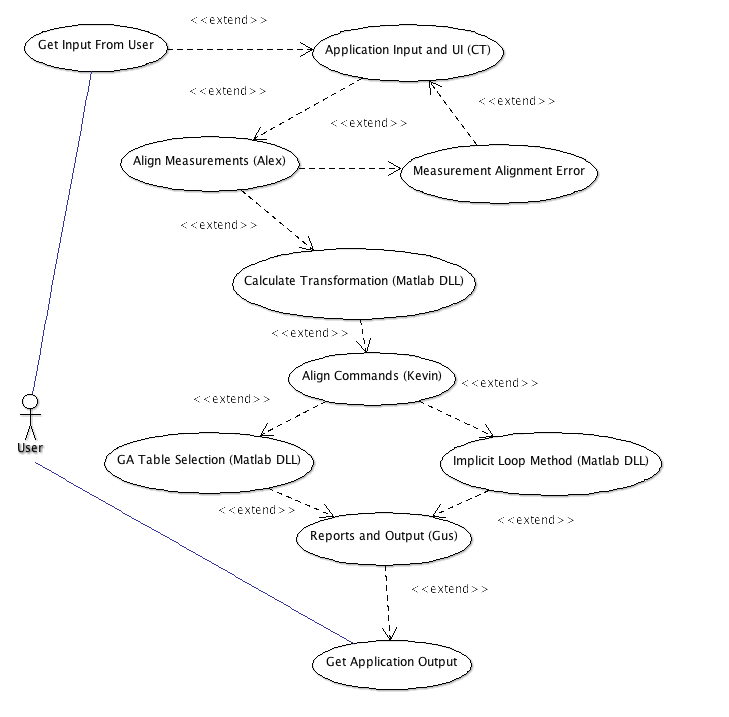
\includegraphics[width=120mm, height=120mm]{UML.png}
\caption{A user interacts with the application by supplying input. The user will receive reports as output. The inputs are processed in the order described by the arrows, starting from the top and ending back at the user.}
\end{figure}

Generation of compensation tables is a linear, multistep process requiring a specific set of input from the user. The required input is a set of long tool measurements, short tool measurements, command positions, machine kinematics, and a tool-specific offset. The tool measurements are then aligned such that they fall within a specific margin of error, before being transformed by a machine configuration. The output from this stage must be aligned to the machine commands; a long or short tool measurement should match a predicted value for a machine command. Finally, this output is supplied to a genetic algorithm and implicit loop method MATLAB  dll. For the final step, the software formats the compensation tables generated by the GA for a specific controller configuration and generates reports from the GA and ILM.

\newpage

\section*{Functional Requirements}
\begin{description}
\item[] [MANDATORY] Parse raw short tool and long tool CSV measurement, tool length, tool offset, and command position data into data structures. [Charles]
\item[] [MANDATORY] Provide GUI for selecting a machine configuration. [Charles]
\item[] [MANDATORY] Indicate progress / current step of the application through the GUI. [Charles]
\item[] [MANDATORY] Parse the input data structure to obtain inputs for each stage of the application. [All]
\item[] [MANDATORY] If the offset between long and short tool measurements is greater than two to three standard deviations, then attempt to align that offset or remove the measurement. [Alex]
\item[] [MANDATORY] If an offset cannot be aligned or too many measurements were not aligned, then throw an error asking for more or new long and short tool measurement data. [Alex]
\item[] [MANDATORY] If the transformation is deemed incorrect, assume that more or new long and short tool measurements are needed and throw an error stating so. [Alex]
\item[] [MANDATORY] Using the aligned measurements, parse the Calculate Transformation MATLAB DLL. [Alex]
\item[] [MANDATORY] Using forward kinematics, align commands such that for a predicted measured position of the machine for a given command, the actual measurement is close to the predicted value. [Kevin]
\item[] [MANDATORY] If an estimated command position and actual command position do not match, discard the measurement. The error should not be greater than $10^{-2}$. [Kevin]
\item[] [MANDATORY] Supply the aligned commands to the Implicit Loop Method and GA Table Selection MATLAB DLLs to obtain output for generating the tables and reports. [Kevin]
\item[] [Mandatory]  Parse controller profile to the GA Table Selection. [Kevin]
\item[] [MANDATORY] Build performance report from the output of the Implicit Loop Method DLL containing a goodness of fit value, calculation time, mean and maximum residual error, and plots of the identified table function. [Gus]
\item[] [MANDATORY] Generate a second performance report from the output of the GA Tables DLL showing the solutions to the genetic algorithm, graph of errors, performance statistics, calculation time, chi squared value, and max/mean residual error. [Gus]
\item[] [MANDATORY] Format the compensation tables populated by the GA algorithm based on a user specified controller type. [Gus]
\end{description}

\section*{Quality Requirements}
\begin{description}
\item[] [DESIRABLE] Use an illustration-driven GUI for selecting a machine configuration. [Charles]
\item[] [DESIRABLE] A brute force technique may be used in repairing long and short tool measurement misalignment. [Alex]
\item[] [DESIRABLE] Integrate a manual discussing how the application transforms its input into output. [Gus]
\end{description}

\section*{Platform Requirements}
\begin{description}
\item[] [MANDATORY] Windows XP and Windows 7
\item[] [MANDATORY] C\# / Microsoft Visual Studio
\item[] [MANDATORY] Mechanism for parsing output from the MATLAB DLL files.
\item[] [MANDATORY] Library for interaction with compiled MATLAB code.
\item[] [MANDATORY] Library to support interaction with Microsoft Office for automatic report generation.
\item[] [MANDATORY] Library to generate plots based on data obtained from MATLAB DLL.
\end{description}

\section*{Process Requirements}
\begin{description}
\item[] [MANDATORY] The development group must provide weekly or bi-weekly updates to clients.
\item[] [MANDATORY] Coding will be managed in sprints, where the team meets to code as a group.
\item[] [MANDATORY] Develop test cases for each step of the application to verify the correctness of output at the end of each processing step. 
\item[] [MANDATORY] Version control must be employed throughout the development process. 

\end{description}

\end{document}



